\section{Adapting Unconditional VAEs into Conditional VAEs}
\label{ch:cigcvae}

\begin{figure*}[b]
  \centering
  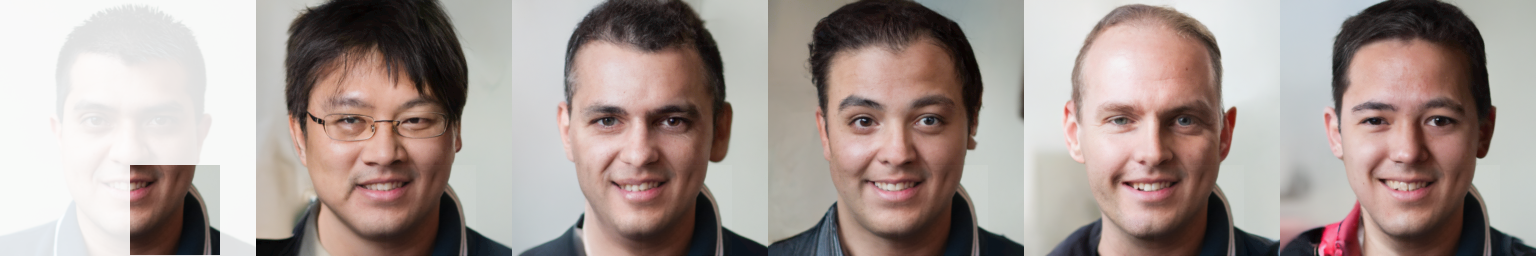
\includegraphics[width=\textwidth]{figs/cigcvae/qual/0_0_patches-4.png}
  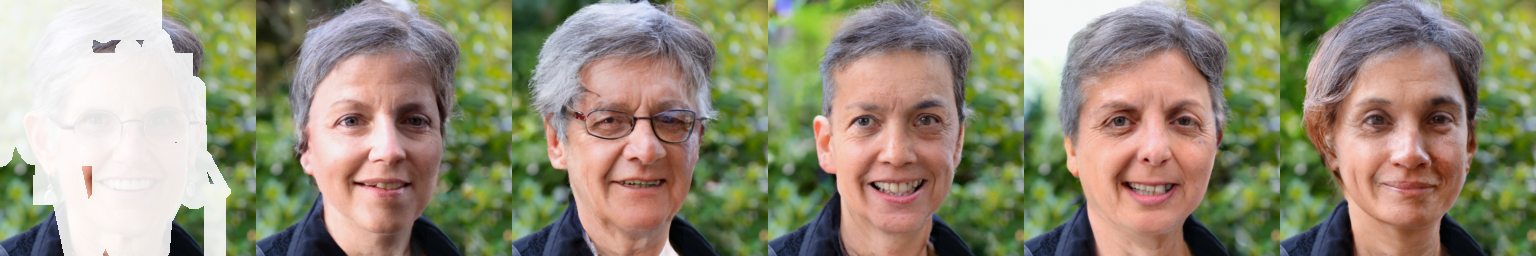
\includegraphics[width=\textwidth]{figs/cigcvae/qual/59_2_3_modddd.png}
  \caption{\textbf{Left column:} Images with most pixels masked out.
    \textbf{Rest:} Completions from IPA, our proposed method.
  }
  \label{fig:cigcvae-headline}
\end{figure*}

A major challenge with applying variational auto-encoders (VAEs) to
high-dimensional data is the typically slow training times. For example,
training a state-of-the-art VAE~\citep{vahdat2020nvae,child2020very} on the
$256\times256$ FFHQ dataset~\citep{karras2019style} takes on the order of 1
GPU-year, but a state-of-the-art generative adversarial network
(GAN)~\citep{lin2021anycost,karras2020analyzing} can be trained on the same
dataset in a matter of GPU-weeks. One hypothesis for the cause of this disparity
is that, whereas the ``mass-covering'' training objective for a VAE forces it to
assign probability mass over the entirety of the data distribution, a GAN can
``cut corners'' by dropping modes~\citep{arora2017gans,arora2017generalization}.

In this thesis we focus on conditional generative models.
% In this chapter we are concerned with conditional generative models, and particularly with the inpainting problem: given an
% input  of a partially blanked-out image, we wish to map to a distribution
% over plausible completions of the image. 
Conditional
GANs~\citep{zheng2019pluralistic,zhao2021large} and conditional
VAEs~\citep{sohn2015learning,ivanov2018variational} have the same disparity in training times that we described for their
unconditional counterparts. We present an approach based on the conditional VAE
framework but, to mitigate the associated slow training times, we design the
architecture so that we can incorporate pretrained unconditional VAEs. We show
that re-using publicly available pretrained models in this way can lead to
training times and sample quality competitive with GANs, while avoiding mode
dropping.


While requiring an existing pretrained model is a limitation, we note that:
\textbf{(\rom{1})} The unconditional VAE need not have been (pre-)trained on the same
dataset as the conditional model; we show unconditional models trained on
ImageNet are suitable for later use with various photo datasets.
\textbf{(\rom{2})} A single unconditional VAE can be used for later training of
conditional VAEs on any desired conditional generation tasks (e.g.~the same
image model may be later used for image completion or image colourisation).
\textbf{(\rom{3})} There is an increasing trend in the machine learning community towards
sharing large, expensively trained models~\citep{wolf2020transformers},
sometimes referred to as foundation models~\citep{bommasani2021opportunities}.
Most of the unconditional VAEs in our experiments use publicly-available
pretrained weights released by \citet{child2020very}. By presenting a use case
for foundation models in image modelling, we hope to encourage even more sharing
of pretrained weights in this domain.

We demonstrate our approach on several conditional generation tasks, but particularly stochastic image completion, the problem of inferring the posterior distribution over images given the observation of a
subset of pixel values. For some applications such as photo-editing the implicit distribution defined by
GANs is good enough. We argue that our approach has substantial advantages when
image completion is used as part of a larger pipeline, and discuss one possible
instance of this in \cref{sec:cigcvae-boed}: Bayesian optimal experimental design (BOED)
for guiding a sensor or hard attention
mechanism~\citep{ma2018eddi,harvey2019near,rangrej2021achieving}. In this case,
missing modes of the posterior over images is likely to lead to bad decisions.
We show that our objective corresponds to the mass-covering KL divergence and so
covers the posterior well. This is supported empirically by results indicating that, not only is the visual quality of our image completions (see \cref{fig:cigcvae-headline}) close to the
state-of-the-art~\citep{zhao2021large}, but our coverage of the ``true''
posterior over image completions is superior to that of any of our baselines.


% \textbf{Contributions} We develop a method to cheaply convert pretrained
% unconditional VAEs into conditional VAEs. The resulting training times and
% sample quality are competitive with GANs, while the models avoid the
% mode-dropping behaviour associated with GANs. Finally, we showcase a possible
% application in Bayesian optimal experimental design that benefits from these
% capabilities.

% \section{Variational Auto-encoders}
% We describe VAEs in terms of three components. \textbf{(\rom{1})} A decoder with
% parameters $\theta\in\Theta$ maps from latent variables $\rvz$ to a distribution
% over data $\rvx$, which we call $p_\theta(\rvx | \rvz; \theta)$. \textbf{(\rom{2})}
% There is a prior over latent variables, $p_\theta(\rvz;\theta)$. This may have
% learnable parameters, which we consider to be part of $\theta$. Together, the
% prior and decoder define a joint distribution, $p_\theta(\rvz, \rvx; \theta)$.
% Finally, \textbf{(\rom{3})} an encoder with parameters $\phi\in\Phi$ maps from
% data to an approximate posterior distribution over latent variables, $q(\rvz|\rvx;
% \phi) \approx p_\theta(\rvz|\rvx; \theta)$. Ideally, $\theta$ would be learned to
% maximise the log likelihood $\logp_\theta(\rvx; \theta) = \log \int
% p_\theta(\rvz, \rvx; \theta) \mathrm{d}\rvz$, averaged over training examples. Since
% this is intractable, $\theta$ and $\phi$ are instead trained jointly to maximise
% an average of the evidence lower-bound (ELBO) over each training example $\rvx
% \sim \pdata(\cdot)$:
% \begin{align}
%   \EX_{\pdata(\rvx)} \left[ \text{ELBO}(\theta, \phi, \rvx) \right] &= \EX_{\pdata(\rvx)} \EX_{q(\rvz|\rvx; \phi)} \left[ \log\frac{p_\theta(\rvz; \theta)p_\theta(\rvx|\rvz; \theta)}{q(\rvz|\rvx; \phi)} \right] \label{eq:eelbo}\\
%                                                                       &= -\mathcal{H}\left[ \pdata(\rvx) \right] - \kl[\big] { \pdata(\rvx)q(\rvz|\rvx; \phi) }{ p_\theta(\rvz, \rvx; \theta) }. \label{eq:elbo-kl-joints}
% \end{align}
% The data distribution's entropy, $\mathcal{H}\left[ \pdata(\rvx) \right]$, is
% typically a finite constant, and this is guaranteed in our experiments where
% $\rvx$ is an image with discrete pixel values. Maximising the above objective
% will therefore drive $p_\theta(\rvz, \rvx; \theta)$ towards
% $\pdata(\rvx)q(\rvz|\rvx; \phi)$, and so the marginal $p_\theta(\rvx; \theta)$
% towards $\pdata(\rvx)$. The KL divergence shown leads to mass-covering
% behaviour from $p_\theta(\rvz, \rvx; \theta)$~\citep{bishop2006pattern} so
% $p_\theta(\rvx; \theta)$ should assign probability broadly over the data
% distribution $\pdata(\rvx)$.
% % This is important since, for the framing of
% % image completion as inference to be well-posed, any observed subsets of image
% % pixels should have non-zero probability under $p_\theta$.
% For notational simplicity in the rest of the paper, parameters $\theta$ and
% $\phi$ are not written when clear from the context.

% Hierarchical
% VAEs~\citep{gregor2015draw,kingma2016improving,sonderby2016ladder,klushyn2019learning}
% partition the latent variables $\rvz$ in a way which has been found to improve the
% fidelity of the learned $p_\theta(\rvx)$, especially for the image
% domain~\citep{vahdat2020nvae,child2020very}. In particular, they define $\rvz$ to
% consist of $L$ disjoint groups, $\rvz_1,\ldots,\rvz_L$. The prior for each $\rvz_l$ can
% depend on the previous groups through the factorisation
% \begin{equation}
%   \label{eq:hierarchical-prior}
%   p_\theta(\rvz) = \prod_{l=1}^L p_\theta(\rvz_l|\rvz_{<l}).
% \end{equation}
% where $\rvz_{<l}$ is the null set for $l=1$ and $\{\rvz_1,\ldots,\rvz_{l-1}\}$
% otherwise. \cref{fig:cigcvae-hierarchical-vae} shows the hierarchical VAE architecture
% we base this work on, in which the dependency of the prior for each $\rvz_l$ on
% $\rvz_{<l}$ is maintained via the decoder's hidden state $h_l$. The distribution
% produced by the encoder for each $\rvz_l$ also depends on the previous hidden
% state $h_{l-1}$ and so factorises as
% $q(\rvz|\rvx) = \prod_{l=1}^L q(\rvz_l|\rvz_{<l}, \rvx)$. We will parameterise
% $p_\theta(\rvz_l|\rvz_{<l})$ and $q(\rvz_l|\rvz_{<l}, \rvx)$ as diagonal
% Gaussian distributions, as is common for hierarchical
% VAEs~\citep{sonderby2016ladder,vahdat2020nvae,child2020very}.

\begin{figure*}[t]
  \centering
  \begin{subfigure}[b]{.32\textwidth}
    \centering
    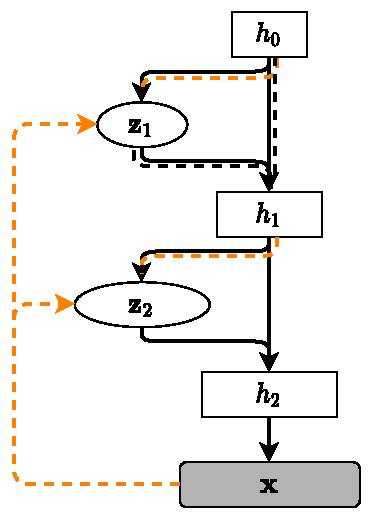
\includegraphics[height=3.8cm]{figs/cigcvae/arch_small-standard.pdf}
    \caption{Estimating ELBO.}
    \label{fig:cigcvae-hierarchical-vae}
  \end{subfigure}
  \begin{subfigure}[b]{.32\textwidth}
    \centering
    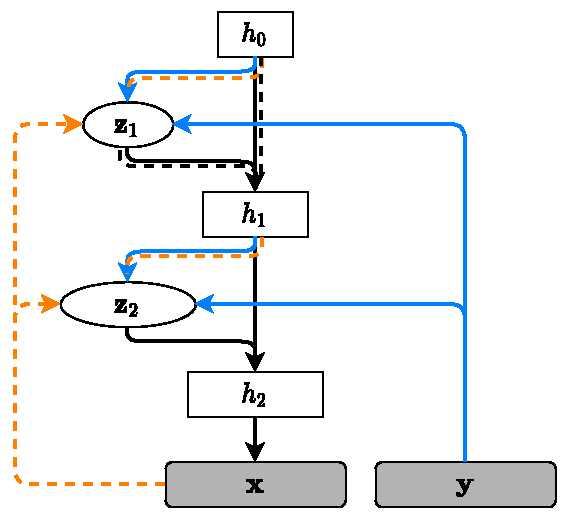
\includegraphics[height=3.8cm]{figs/cigcvae/arch_small-forward.pdf}
    \caption{Estimating $\mathcal{O}_\mathrm{for}$.}
    \label{fig:cigcvae-forward-arch}
  \end{subfigure}
  \begin{subfigure}[b]{.32\textwidth}
    \centering
    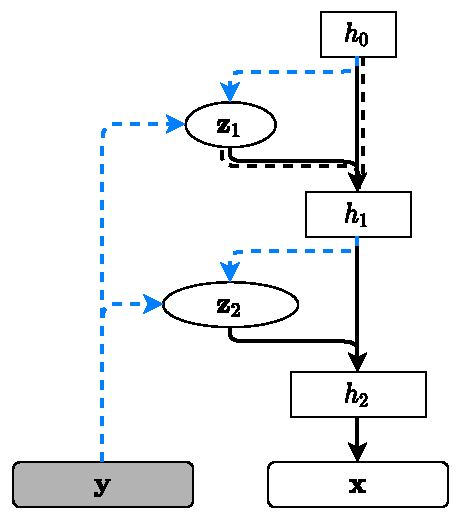
\includegraphics[height=3.8cm]{figs/cigcvae/arch_small-sampling.pdf}
    \caption{Sampling $\rvx\sim p_{\theta,\psi}(\cdot|\rvy)$.}
    \label{fig:cigcvae-reverse-arch}
  \end{subfigure}
  \vspace{-1mm}
  \caption{A hierarchical VAE architecture with $L=2$ layers of latent
    variables. Part (a) illustrates the computation of the ELBO for an
    unconditional VAE; part (b) illustrates the computation of our training
    objective $\mathcal{O}_\mathrm{for}$; and part (c) illustrates the drawing
    of conditional samples. The encoder is shown in orange; the prior and the
    decoder (which maintains a deterministic hidden state $h_{l}$) are both
    shown in black; and the partial encoder is shown in blue. The computation
    graph needed to sample $\rvz$ in each case is drawn with dashed lines, and
    the remainder of the computation graph is drawn with solid lines.}
  \label{fig:cigcvae-conditional-architectures}
  \vspace{-2mm}
\end{figure*}

\section{Amortized Inference in a Pretrained Artifact}
To convert an unconditional VAE architecture to a conditional architecture, we
introduce a \textit{partial encoder} with parameters $\psi\in\Psi$. \todo{partial encoder = conditional prior from earlier. note we call it a partial encoder because of its similarity to encoder architecture}
Given a conditioning input $\rvy$ (which could be, e.g., an image with some
pixels masked out in the case of inpainting), the partial encoder defines an
approximate posterior over the latent variables,
$p_\psi(\rvz|\rvy)$.
%
Since the conditional generation task is
to approximate $\pdata(\rvx|\rvy)$, we use the partial encoder to define
\begin{equation}
  \label{eq:marginal-image-posterior}
  p_{\theta,\psi}(\rvx|\rvy) := \int p_\theta(\rvx|\rvz)q_\psi(\rvz|\rvy) \mathrm{d}\rvz
\end{equation}
with learnable parameters $\theta$ and $\psi$. We can sample from
$p_{\theta,\psi}(\rvx|\rvy)$ by sampling $\rvz\sim p_\psi(\cdot|\rvy)$ and then
$\rvx\sim p_\theta(\cdot|\rvz)$ as shown in \cref{fig:cigcvae-reverse-arch}. This defines
a conditional VAE architecture which, unique amongst related work with
high-dimensional $\rvx$ and
$\rvy$~\citep{sohn2015learning,zheng2019pluralistic,ivanov2018variational,wan2021high},
has a decoder $p_\theta(\rvx|\rvz)$ with no dependence on $\rvy$. This
decoder can therefore use an architecture identical to that of an unconditional
VAE and also, as we will show later, re-use unconditional VAE weights.

\todo{reference bakground in this paragraph?}
We now introduce some notation before describing our method further. Let the
distribution of paired data be $\pdata(\rvx, \rvy)$, and recall that
training an unconditional VAE matches two joint distributions: the distribution
of unconditional samples, $p_\theta(\rvz, \rvx)$; and the distribution
resulting from sampling data $\rvx$ and then encoding it, $\pdata(\rvx)q(\rvz|\rvx)$.
% encoding samples from the dataset,
We define
extensions of each to include $\rvy$:
\begin{align}
  p_\theta(\rvz, \rvx, \rvy) &= p_\theta(\rvz)p_\theta(\rvx|\rvz)\pdata(\rvy|\rvx), \label{eq:pmodel} \\
  q_\phi(\rvz, \rvx, \rvy) &= \pdata(\rvx, \rvy)q_\phi(\rvz|\rvx), \label{eq:r}
\end{align}
% alternatively:
% \begin{align}
%   p_\theta(\rvz, \rvx, \rvy) &= p_\theta(\rvz)p_\theta(\rvx|\rvz)\pdata(\rvy|\rvx), \label{eq:pmodel} \\
%   q_\phi(\rvz, \rvx, \rvy) &= \pdata(\rvx, \rvy)q_\phi(\rvz|\rvx), \label{eq:r}
% \end{align}
where $\pdata(\rvy|\rvx)$ is a (potentially intractable) conditional
distribution under $\pdata(\rvx, \rvy)$.
%
Note that $p_\theta(\rvz, \rvx, \rvy)$ and $q_\phi(\rvz, \rvx, \rvy)$ are exactly the two distributions matched by the unconditional VAE
objective in \cref{eq:elbo-kl-joints} with an additional factor of
$\pdata(\rvy|\rvx)$.
%
Therefore, if the unconditional VAE represented by $\theta$ and $\phi$ is well
trained, $p_\theta(\rvz, \rvx, \rvy)$ and
$q_\phi(\rvz, \rvx, \rvy)$ will be close. From now on, we will use
$p_\theta$ and $r$ to refer to any marginals and conditionals of the above
joint distributions, with the specific marginal or conditional clear from
context.

\subsection{Training objective}

Our training objective, previously used for training conditional
VAEs~\citep{sohn2015learning,ivanov2018variational} and neural
processes~\citep{garnelo2018neural}, is
\begin{align}
  \label{eq:forward-elbo}
  \mathcal{O}_\mathrm{for}(\theta, \phi, \psi) &= \EX_{\pdata(\rvx, \rvy)} \EX_{q_\phi(\rvz|\rvx)} \left[ \log \frac{p_\theta(\tildeI|\rvz)p_\psi(\rvz|\rvy)}{q_\phi(\rvz|\rvx)} \right] \\
  &\leq \EX_{\pdata(\rvx, \rvy)} \left[ \log p_{\theta,\psi}(\tildeI{}|\rvy) \right]
\end{align}
where $\tilde{\rvx}$ is the part of $\rvx$ we wish to predict. In general we can
set $\tildeI{}:=\rvx$ but for inpainting define $\tildeI{}$ to consist of only
the dimensions of $\rvx$ not observed in $\rvy$, abusing notation by
ignoring the implication that $\tildeI{}$ is formally a function of $\rvy$
as well as $\rvx$. Our architectures have pixel-wise independent
likelihoods so $p_\theta(\tildeI{}|\rvz)$ is tractable in either case. \Cref{eq:forward-elbo}
lower-bounds $\log p_{\theta,\psi}(\tildeI{}|\rvy) $ similarly to how the ELBO of
an unconditional VAE lower-bounds $\log p_\theta(\rvx)$. The major difference
is that the prior, $p_\theta(\rvz)$, is replaced by $p_\psi(\rvz|\rvy)$.
This is reflected in \cref{fig:cigcvae-forward-arch} where each $\rvz_l$ is conditioned
on $\rvy$ via the partial encoder.
%
Similar to standard estimators for an unconditional hierarchical VAE's ELBO,
reduced-variance estimates of \cref{eq:forward-elbo} can be obtained by
computing KL divergences between $q(\rvz_l|\rvz_{<l},\rvx)$ and
$p_\psi(\rvz_l|\rvz_{<l},\rvy)$ analytically for each layer $l$ (see
\cref{supp:cigcvae-kl-estimates} for details).

We are particularly interested in the properties of the learned partial encoder.
Recall the joint distribution $q_\phi(\rvz, \rvx, \rvy) = \pdata(\rvx,
\rvy)q_\phi(\rvz|\rvx)$. Then $q_\phi(\rvz|\rvy)$ is the intractable
posterior given by marginalising out $\rvx$ and conditioning on $\rvy$. We
find that fitting $\psi$ to maximise $\mathcal{O}_\mathrm{for}(\theta,
\phi, \psi)$ is equivalent to minimising the mass-covering KL divergence
from $q_\phi(\rvz|\rvy)$ to $p_\psi(\rvz|\rvy)$. We formalise
this statement in the following theorem, which is proven in
\cref{proof:forward-kl}.
\begin{theorem} \label{theorem:forward-kl} For any set $\Psi$ of
  permissible values of $\psi$, and for any $\theta\in\Theta$ and
  $\phi\in\Phi$,
  \begin{equation} \label{eq:forward-theorem}
    \argmax_{\psi \in \Psi} \mathcal{O}_\mathrm{for}(\theta, \phi, \psi) = \argmin_{\psi \in \Psi} \EX_{\pdata(\rvy)} \left[ \kl[\big]{ q_\phi(\rvz|\rvy) }{ p_\psi(\rvz|\rvy) } \right].
  \end{equation}
\end{theorem}
Due to the mass-covering properties of this ``forward'' KL
divergence~\citep{bishop2006pattern}, this theorem indicates that 
the learned $p_\psi(\rvz|\rvy)$ should have good coverage of all
modes of $q_\phi(\rvz|\rvy)$. Intuitively, the resulting diverse samples of
latent variables $\rvz\sim p_\psi(\cdot|\rvy)$ should lead to
diverse samples of $\tildeI{} \sim p_\theta(\cdot|\rvz)$ which cover the
``true'' posterior $\pdata(\tildeI{}|\rvy)$. We formalise this in
\cref{proof:forward-kl} by showing that maximising $\mathcal{O}_\mathrm{for}$
also minimises an upper-bound on a KL divergence in $\tildeI{}$-space.

\subsection{Faster training with a pretrained VAE}
To justify using weights trained as part of an unconditional VAE we present
\cref{theorem:joint-training}.
%
\begin{theorem} \label{theorem:joint-training} Assume that we have a
  sufficiently expressive encoder and decoder that there exist parameters
  $\optimal{\theta}\in\Theta$ and $\optimal{\phi}\in\Phi$ which make the
  unconditional VAE objective (\cref{eq:eelbo}) equal to its upper bound of
  $-\mathcal{H}\left[ \pdata(\rvx) \right]$. Assume also that $\tildeI{}$ is
  defined such that there is a mapping from $(\tildeI{},\rvy)$ to $\rvx$ and
  that the mutual information ${\mutinf{} := \EX_{p_{\theta^*}(\tildeI{}, \rvy,
      \rvz)} \left[ \log \frac{p_{\theta^*}(\tildeI{},\rvy|\rvz)
      }{ p_{\theta^*}(\tildeI{}|\rvz)p_{\theta^*}(\rvy|\rvz) }
    \right]}$ is zero (see discussion below). Then, given a sufficiently expressive
  partial encoder,
  \begin{equation} \label{eq:joint-training}
    \max_{\psi} \mathcal{O}_\mathrm{for}(\optimal{\theta}, \optimal{\phi}, \psi) = \max_{\theta, \phi, \psi} \mathcal{O}_\mathrm{for}(\theta, \phi, \psi).
  \end{equation}
\end{theorem}
This is proven in \cref{proof:joint-training} and implies that we can use values
of $\theta$ and $\phi$ learned using the unconditional VAE objective. Then to
train a conditional generative model we need only optimise $\psi$. This
leads to faster convergence, as well as faster training iterations since we only
need to compute gradients for, and perform update steps on, the partial
encoder's parameters $\psi$. For all of our experiments in
\cref{sec:cigcvae-experiments} we use pretrained models released by
\citet{child2020very}, leveraging between 2 GPU-weeks and 1 GPU-year of
unconditional VAE training for each dataset. We name our method IPA (Inference
in a Pretrained Artifact).

\textcolor{black}{\Cref{theorem:joint-training} relies on the assumption that
  the mutual information $\mutinf$ is zero; as we argue in
  \cref{proof:joint-training}, this is true for inpainting and also
  ``approximately'' holds if $\rvy$ consists of high-level features. When
  lower level features are conditioned on, e.g.~for super-resolution, there may
  be a significant gap between the left- and right- hand sides of
  \cref{eq:joint-training}. } \Cref{theorem:joint-training} also applies only if
the unconditional VAE parameters are learned on the same dataset as the
conditional VAE is trained on; otherwise there will be a mismatch between the
form of $\pdata$ used in \cref{eq:eelbo} to fit $\theta^*$ and $\phi^*$, and
the form of $\pdata$ implicit in the $\mathcal{O}_\mathrm{for}$ objective.
However we find empirically that we can use unconditional VAE parameters trained
on ImageNet~\citep{deng2009imagenet} with IPA on several other photo datasets.

\begin{table*}
  \tiny
  \caption{Image completion results. Best performance is shown in \textbf{bold},
    and second best is \underline{underlined}. In the last row, $t$ denotes the
    ``temperature'' parameter \citep{child2020very}.}
  \label{tab:cigcvae-results-completion}
  \centering
  \begin{tabular}{lccccccccc}
    \toprule
    \multicolumn{1}{r}{} & \multicolumn{3}{c}{CIFAR-10}  & \multicolumn{3}{c}{ImageNet-64}  & \multicolumn{3}{c}{FFHQ-256} \\
    \cmidrule(r){2-4} \cmidrule(r){5-7} \cmidrule(r){8-10} % \cmidrule(r){6-7} \cmidrule(r){8-9}
    Method        & \quad FID$\downarrow$ \quad     & P-IDS$\uparrow$  & LPIPS-GT$\downarrow$ & \quad FID$\downarrow$ \quad    & P-IDS$\uparrow$  & LPIPS-GT$\downarrow$& \quad FID$\downarrow$ \quad    & P-IDS$\uparrow$  & LPIPS-GT$\downarrow$ \\
    \midrule
    ANP                        & 30.03               & ~~5.86              & .0447                         & -                 & -                 & -                & 39.95              & ~~0.93              & .256 \\
    CE                         & 21.92               & ~~4.77              & .0628                         & -                 & -                 & -                & 39.02              & ~~0.66              & .267 \\
    RFR                        & 44.35               & ~~2.76              & .0883                         & -                 & -                   & -              & 72.50              & ~~0.46              & .271 \\
    PIC                        & 14.73               & ~~5.95              & .0332                         & 40.0              & 0.24                & .170           & 11.60              & ~~2.76              & .169 \\
    CoModGAN                   & ~~\underline{9.65}  & 11.59               & .0326                         & 20.2              & ~~7.09              & .160           & ~~\textbf{2.33}    & \textbf{13.57}      & .143 \\
    IPA-R                      & 19.21               & ~~8.56              & .0330                         & 28.8              & 6.46                & .166           & ~~8.82             & ~~4.56              & .142 \\
    IPA (ours)                 & 10.50               & \underline{13.24}   & \textbf{.0262}                & \underline{18.9}  & ~~\underline{9.20}  & \underline{.138}  & ~~3.93             & ~~7.79              & \underline{.123} \\
    IPA$_{t=0.85}$ (ours)      & ~~\textbf{8.61}     & \textbf{14.19}      & \underline{.0263}             & \textbf{15.1}     & \textbf{11.26}    & \textbf{.133}     & ~~\underline{3.29} & ~~\underline{8.50}  & \textbf{.117} \\
    \bottomrule
  \end{tabular}
  \vspace{-1em}
\end{table*}


\section{Experiments} \label{sec:cigcvae-experiments}

\paragraph{Comparison to image completion baselines}

We create an IPA image completion model based on the VD-VAE unconditional
architecture~\citep{child2020very}, and evaluate it for image completion on
three datasets: CIFAR-10~\citep{krizhevsky2009learning},
ImageNet-64~\citep{deng2009imagenet}, and FFHQ-256~\citep{karras2019style}. We
compare against four baselines: Co-Modulated Generative Adversarial Networks
(CoModGAN)~\citep{zhao2021large}; Pluralistic Image Completion
(PIC)~\citep{zheng2019pluralistic}; Context Encoders
(CE)~\citep{pathak2016context}; and Attentive Neural Processes
(ANP)~\citep{kim2019attentive}. We also considered two further methods: we show
samples from VQ-VAE~\citep{peng2021generating} (but not quantitative results
which were too slow to compute because it takes roughly one minute per test
image); and we report results for Recurrent Feature Reasoning for Image
Inpainting (RFR)~\citep{li2020recurrent} with the caveat that it is slow to run
on images with many missing pixels and so, although it used a similar
computational budget to the other models, its training did not converge.

Given pretrained unconditional VAE parameters, IPA is faster to train than the
best-performing baseline, CoModGAN. IPA takes 115 GPU-hours to train on
CIFAR-10, and under 7 GPU-weeks on FFHQ-256. The CoModGAN models are trained for
270 GPU-hours and 8 GPU-weeks respectively. We provide more training details in
\cref{supp:cigcvae-exp-details}.

We report the FID~\citep{heusel2017gans} and P-IDS~\citep{zhao2021large} metrics
between a set of sampled completions from each method and a reference set.
Broadly speaking, these measure the sample quality.
%
To investigate how well the samples capture all modes of
$\pdata(\rvx|\rvy)$, we also report the LPIPS-GT. We compute this using
LPIPS~\citep{zhang2018unreasonable}, a measure of distance between two images.
Specifically, we compute the average over test pairs $(\rvx, \rvy)$ of
$\min_{k=1}^K(\text{LPIPS}(\rvx^{(k)} , \rvx))$, with each $\rvx^{(k)} \sim
p_{\theta,\psi}(\cdot | \rvy)$. As $K \rightarrow \infty$, the LPIPS-GT should tend
to zero if the ground truth is always within the support of
$\pcomp(\rvx|\rvy)$. If not, the LPIPS-GT will remain high, penalising
methods which miss modes of the posterior. We use $K=100$. We confirm in
\cref{supp:cigcvae-additional-results} that the LPIPS-GT correlates with diversity
metrics used by related work~\citep{zhu2017toward,li2020multimodal}.


For the image completion tasks, we sample from $\pdata(\rvx, \rvy)$ by
first sampling an image $\rvx$ from the dataset, and then sampling an
image-sized binary mask $m$ from the freeform mask distribution used by
\citet{zhao2021large}, which is itself based on \citet{yu2018generative}. We
then set $\rvy = \texttt{concatenate}(\rvx \odot m, m)$. Here, $\odot$ is a
pixel-wise multiplication operation which removes information from the missing
pixels. The concatenation is performed along the channel dimension and makes it
possible to distinguish between unobserved pixels and zero-valued pixels.

For evaluation, since the number of observed pixels in freeform masks varies
considerably, we follow \citet{zhao2021large} and partition the mask
distribution by conditioning the procedure to return a mask with the proportion
of pixels observed within some range (0-20\%, 20-40\%, and so on) and report
metrics for each range separately in \cref{fig:cigcvae-metrics} (or
\cref{supp:cigcvae-additional-results} for ImageNet-64). To summarise the
overall performance in \cref{tab:cigcvae-results-completion}, we sample masks from a
uniformly-weighted mixture distribution over these five partitions. In terms of
the LPIPS-GT scores in \cref{tab:cigcvae-results-completion}, IPA outperforms the best
baselines by roughly 20\%. \Cref{fig:cigcvae-metrics} shows that there is an improvement
for any proportion of observed pixels. This suggests that IPA produces reliably
diverse samples with good coverage of $\pdata(\rvx|\rvy)$. In contrast, we
believe that the GAN-based approaches occasionally miss modes of
$\pdata(\rvx|\rvy)$ and can therefore fail to capture the ground-truth.
This hypothesis is supported by samples from CoModGAN we display in
\cref{supp:cigcvae-comodgan-failure}. In terms of sample fidelity, as measured by both
FID and P-IDS, IPA outperforms all baselines on CIFAR-10 when over $40\%$ of the
image is observed, and on ImageNet-64 when over $20\%$ is observed. IPA comes
second to CoModGAN when less is observed and on FFHQ-256.

\begin{figure*}[t]
  %\vspace{-.1cm}
  \centering
  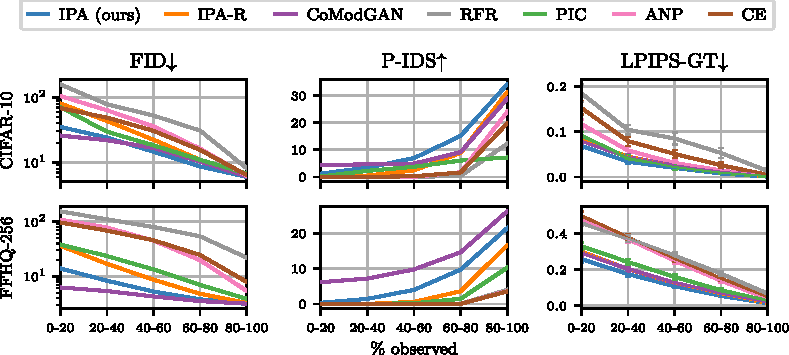
\includegraphics[width=\textwidth]{figs/cigcvae/metrics}
  %\vspace{-.6cm}
  \caption{Test metrics on CIFAR-10 and FFHQ-256, plotted as a function of
    the mask distribution. Error bars on LPIPS-GT show the standard error of our
    estimate for a single trained network.}
  \label{fig:cigcvae-metrics}
  \vspace{-.5cm}
\end{figure*}


\paragraph{Edges-to-photos}
We provide an additional demonstration of IPA on the Edges2Shoes and
Edges2Handbags datasets~\citep{isola2016image}, where the task is to generate an
image conditioned on the output of an edge detector applied to that image. We
downsample the datasets to $64\times64$ so that we can use unconditional VAEs
pretrained on ImageNet~\citep{deng2009imagenet} at this resolution by
\citet{child2020very}. We show in \cref{fig:cigcvae-training} that IPA is useful for
these tasks, and provide further discussion below. The images generated are
diverse and photorealistic, as shown in \cref{supp:cigcvae-image-samples}.

\paragraph{Effectiveness of pretraining}
We now seek to determine how important the pretrained unconditional VAE weights
are to IPA. We compare IPA with conditional VAEs which use IPA's architecture
but are trained from scratch, which we will refer to as ``from-scratch''
baselines. That is, $\theta$ and $\phi$ are randomly initialised and trained to
maximise \cref{eq:forward-elbo} (with $\tildeI{} := \rvx$) along with
$\psi$.
%
With an infinite training budget, the end-to-end training of the from-scratch
baselines is likely to lead them to outperform any IPA models. Nevertheless it
is apparent from \cref{fig:cigcvae-training} that, in the more realistic situation of a
finite training budget, using IPA can be beneficial. This is the case even for
training budgets of up to a few GPU-weeks on the relatively small CIFAR-10
dataset. In fact, even with only a couple of days of training, IPA on CIFAR-10
(with CIFAR-10 pretraining) achieves better FID and ELBO scores than the
from-scratch baseline trained for several weeks. For ImageNet-64, IPA performs
better after 4 hours than the from-scratch baseline does after a week.
%
For Edges2Handbags and Edges2Shoes, training with IPA for 2 days yields
performance similar to or better than training with the from-scratch baseline
for 1 week, as measured by the ELBO. This is despite IPA on these datasets using
a trained ImageNet-64 model rather than a model pretrained on those specific
datasets, supporting our suggestion that the dataset used for pretraining need
not exactly match what IPA is then trained on.
%
Measured by the FID score, IPA's performance is even more appealing: wherever
ELBOs are similar between IPA and the from-scratch baselines, IPA achieves a
significantly better FID score.
%
We see that IPA pretrained on ImageNet is less effective for CIFAR-10
than it is for the edges-to-photos datasets, but it improves on the from-scratch
baseline in terms of ELBO for the first 30 hours of training, and in terms of
FID until the from-scratch baseline is trained for several weeks.

\paragraph{An alternative training objective}
In \cref{tab:cigcvae-results-completion} and \cref{fig:cigcvae-metrics}, we report results for
IPA-R, a variation of IPA with a different training objective corresponding to a
mode-seeking KL divergence. IPA almost always outperforms IPA-R, but we
nonetheless provide a full description of IPA-R in \cref{supp:cigcvae-ipa-r}.

\begin{figure*}[t]
  \vspace{-.1cm}
  \centering
  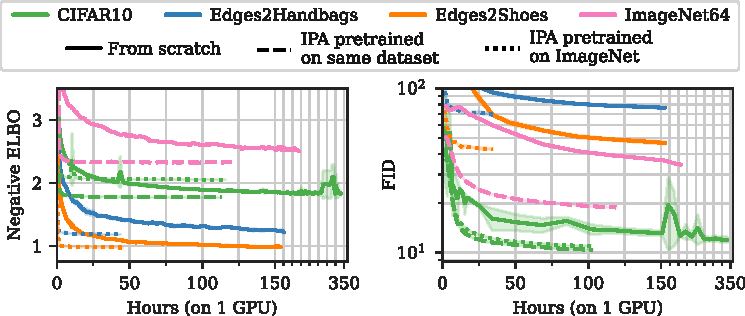
\includegraphics[scale=1]{figs/cigcvae/training-both}
  \caption{ELBO (\cref{eq:forward-elbo} computed with $\tildeI{} := \rvx$) and
    FID during training using IPA with pretraining on the same dataset, IPA with
    pretraining on ImageNet, and when trained from scratch. Error bars show
    standard deviations computed with 3 runs. IPA makes training faster and
    lower-variance.}
  \label{fig:cigcvae-training}
  \vspace{-.3cm}
\end{figure*}




\section{Inpainting for Bayesian Experimental Design} \label{sec:cigcvae-boed}

In this section, we explore a potential application for stochastic image completion that
requires a faithful representation of the posterior $\pdata(\rvx|\rvy)$.
%
In particular, we consider whether it is possible to automatically target a
chest x-ray at areas most likely to reveal abnormalities. This could avoid the
need to scan the entire chest and so bring benefits including reducing the
patient's radiation exposure.
%
While doing so is not possible with standard x-ray machines (which do not take
multiple scans consecutively), and would need to be extensively validated before
use in a clinical setting, we believe this is a worthwhile avenue to explore.
%
Specifically, our imagined system performs a series of x-ray scans, each
targeted at only a small portion of the area of interest. We can select the
coordinates $\coord_t = (x_t, y_t)$ of the location to scan at each step $t$, and
this selection can be informed by what was observed in the previous scans. The
task we consider is how to select $\coord{}_t$ to be maximally informative. In
particular, assume we wish to infer a variable $v$ representing, e.g., whether
the patient has a particular illness. Bayesian optimal experimental design
(BOED)~\citep{chaloner1995bayesian} provides a framework to select a value of
$\coord{}_t$ that is maximally informative about $v$.
%
It involves taking a Bayesian perspective on the problem of estimating $v$. We
have one posterior distribution over $v$ after taking scans at
$\coord{}_1,\ldots,\coord{}_{t-1}$ and another (typically lower entropy) distribution after
conditioning on a scan at $\coord{}_t$ as well.
%
The \textit{expected information gain}, or EIG, quantifies the utility of the
choice of $\coord{}_t$ as the expected difference in entropy between these two
distributions. Using BOED involves estimating the EIG and selecting the scan
location, $\coord{}_t$, to minimise it.

\begin{figure}[t]
  \centering
  \hspace{-.75cm}
  \begin{minipage}{.4\textwidth}
    \centering
    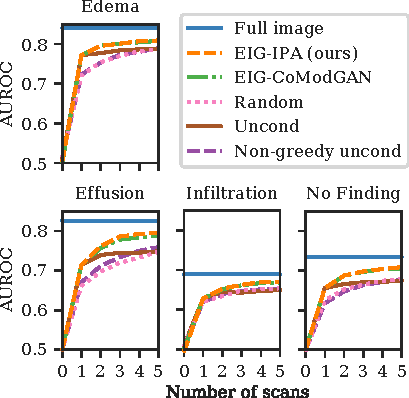
\includegraphics[scale=.77]{figs/cigcvae/boed-auroc-curve-rearranged}
  \end{minipage}
  ~
  \begin{minipage}{0.54\textwidth}
    \centering
    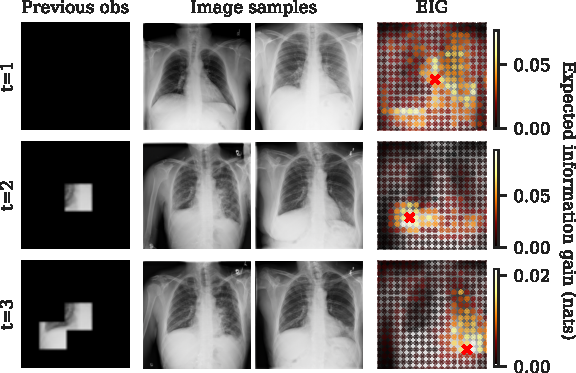
\includegraphics[scale=.77]{figs/cigcvae/shrunk-boed-vis}
  \end{minipage}
  \caption{\textbf{Left:} Classification AUROC scores after $1,\ldots,5$ scans
    chosen with each method. Scores for the ``EIG-'' methods more quickly approach the
    upper bound achieved by processing the full image. \textbf{Right:}
    Visualisation of BOED used to select three scan locations for diagnosing
    `Effusion'. The left column shows the observations made prior to each time
    step. We then show samples from IPA (or the dataset when $t=1$). The
    rightmost column shows the EIG overlaid on the pixel-space average of
    sampled images, with the optimal $\coord{}_t$ marked by a red cross.}
  \label{fig:cigcvae-boed}
  \vspace{-.4cm}
\end{figure}



We use an estimator for the EIG similar to that of \citet{harvey2019near}. It
requires two components:
\textbf{(\rom{1})} A neural network trained to classify $v$ given a series of
scans at locations $\coord{}_1,\ldots,\coord{}_t$. This outputs a classification distribution
which we denote $g(v|f_{\coord{}_1,\ldots,\coord{}_t}(\rvx))$, where $f_{\coord{}_1,\ldots,\coord{}_t}$ is a
function mapping from an image to the values of the pixels observed by scans at
$\coord{}_1,\ldots,\coord{}_t$. We use this classification distribution as an approximation of
the posterior over $v$, whose entropy we attempt to minimise by performing BOED.
\textbf{(\rom{2})} A method for sampling image completions conditioned on some
observed pixel values $f_{\coord{}_1,\ldots,\coord{}_{t-1}}(\rvx)$. \citet{harvey2019near}
used a “stochastic image completion” module which contributed significant
complexity to their method. We entirely replace this with IPA.

Let the pixel values observed so far be $\rvy_{\coord{}_1,\ldots,\coord{}_{t-1}} =
f_{\coord{}_1,\ldots,\coord{}_{t-1}}(\rvx)$ for a latent image $\rvx$. Given these, we
estimate the EIG of location $\coord{}_t$ as
\begin{align}
  \label{eq:new-eig}
  \text{EIG}(\coord{}_t;& \rvy_{\coord{}_1,\ldots,\coord{}_{t-1}}) \approx \overbrace{\mathcal{H} \left[ \frac{1}{N} \sum_{n=1}^N g(\cdot|f_{\coord{}_1,\ldots,\coord{}_t}(\rvx^{(n)})) \right]}^{\text{entropy after $t-1$ scans}} - \overbrace{\frac{1}{N} \sum_{n=1}^N  \mathcal{H} \left[ g(\cdot|f_{\coord{}_1,\ldots,\coord{}_t}(\rvx^{(n)})) \right]}^{\text{expected entropy after $t$ scans}},
\end{align}
where $\rvx^{(1)},\ldots,\rvx^{(N)}$ are sampled image completions from IPA
given $\rvy_{\coord{}_1,\ldots,\coord{}_{t-1}}$. In \cref{sec:cigcvae-supp-boed} we report
hyperparameters, provide further details of our EIG estimator, and compare it to
the estimators used in related work. To select $\coord{}_t$, we simply estimate
$\text{EIG}(\coord{}_t; \rvy_{\coord{}_1,\ldots,\coord{}_{t-1}})$ for many different values of
$\coord{}_t$ and select the value which maximises it. This process of selecting $\coord{}_t$
and then taking a scan is repeated for each $t=1,\ldots,T$.

We experiment on the NIH Chest X-ray 14 dataset~\citep{wang2017chestx} at
$256\times256$ resolution.
%
%
% , in which each image is labelled with the presence or
% absence of 14 illnesses. We set $v$ to be a binary label indicating the
% presence/absence of a particular illness. A simple extension, with appropriate
% training data, could be to define $v$ to be the severity of an illness, and
% therefore also infer the severity.
%
We simulate a scanner which returns a $64 \times 64$ pixel patch from this
image, and the task is to diagnose the binary presence or absence of an illness.
We run separate experiments diagnosing each of edema, effusion, infiltration and
``no finding'' (an additional label meaning there are no diagnosed illnesses).
With appropriate data, this framework could be extended to also infer the
severity of a given illness.
%
We envisage BOED being used to select scan locations for an x-ray without
necessarily performing an automated diagnosis. However, to quantify the
informativeness of the chosen locations, \cref{fig:cigcvae-boed} shows the results of
using $g$ to perform a diagnosis, or classification, based on the chosen scan
locations.
%
Since the conditional distribution $g$ (used to estimate the EIG) depends on
which illness we are classifying, the choice of scan locations is different in
each case.
%
We compare against a baseline where the image completion is performed by
CoModGAN (our best-performing image completion baseline) rather than IPA, as
well as numerous baselines which choose scan locations without image
completion; see \cref{sec:cigcvae-supp-boed} for details.

Our method (denoted EIG-IPA) narrowly but consistently outperforms EIG-CoModGAN.
%
% We hypothesise that this is due to CoModGAN's tendency to sometimes produce
% almost no diversity in its completions, even when the observed pixels are
% uninformative.
%
We hypothesise that this is due to the aforementioned tendency of CoModGAN to
sometimes collapse to a single mode of the posterior, and exhibit an example of
this behaviour on the x-ray dataset in \cref{supp:cigcvae-image-samples}. In the BOED
context, such ``overconfident'' image completion could lead to salient scan
locations being ignored. Nonetheless, both EIG-IPA and EIG-CoModGAN
significantly outperform the other baselines, giving performance much closer to
the upper bound of a CNN with access to the entire image. Another benefit of the
``EIG-'' approaches is that the choice of scan locations is highly
interpretable; we can see why a particular location was chosen with
visualisations similar to the right of \cref{fig:cigcvae-boed}. This shows the sampled
images $\rvx^{(n)}$ and the estimated EIG for each $\coord{}_t$. In \cref{sec:cigcvae-supp-boed}, we
show that we can further quantify the contribution of each $\rvx^{(n)}$ to the
estimated EIG for each $\coord{}_t$.


\section{Related Work}
\paragraph{Inference in pretrained VAEs}
Several prior studies perform conditional generation using a previously trained
unconditional VAE.
%
Like us, \citet{rezende2014stochastic,nguyen2016plug,wu2018conditional} do so
through inference in the VAE's latent space. However, they use non-amortized
inference (Gibbs sampling, variational inference, and MCMC respectively),
leading to slow sampling times for any new $\rvy$.
%
\citet{duan2019pre} learn variational distributions over $\rvz$ for every possible
value of $\rvy$, but this is not possible when $\rvy$ is
high-dimensional or continuous-valued.
%
\citet{yeh2017semantic} fit the latent variables of a GAN given observations,
but this is neither amortized nor probabilistic.
%

\paragraph{Conditional VAEs}
Past research on conditional
VAEs~\citep{sohn2015learning,zheng2019pluralistic,ivanov2018variational,wan2021high}
has generally been unable to take advantage of pretrained weights as we have due
to a difference in architectures: unlike almost all prior work, the IPA decoder
does not receive $\rvy$ as input. The dependence between $\rvy$ and the
decoder's output must therefore be expressed solely through the conditional
distribution over the latent variables, $p_\psi(\rvz|\rvy)$. This is a crucial
difference because it means that the decoder can have exactly the same
architecture as that of an unconditional VAE. This is key to letting us copy the
pretrained weights of an unconditional VAE to speed up training. The exception
to the above is \citet{ma2018eddi} who, like us, use a conditional VAE decoder
with no dependence on $\rvy$. Their training objective and use case are
different, however, and they do not consider using pretrained models or use an
architecture which can scale to photorealistic images. Leveraging unconditional
VAEs lets us drastically reduce the computational budget required to train a
conditional VAE. We believe that this paper is the first to demonstrate
photorealistic image completion with conditional VAEs at resolutions as high as
$256\times256$.
% 
Another benefit of the decoder having no dependence on $\rvy$ is that it
makes impossible the ``posterior collapse'' phenomenon discussed by
\citet{zheng2019pluralistic}, in which a conditional VAE's decoder learns to
ignore $\rvz$ and produce outputs conditioned solely on $\mathbf{y}$.


\paragraph{Image completion}
Early work on image completion, both
before~\citep{bertalmio2000image,bertalmio2001navier,ballester2001filling,levin2003learning,criminisi2003object}
and after~\citep{kohler2014mask,ren2015shepard} deep learning became the
dominant approach, aimed to deterministically fill in missing pixels in images.
Even many methods incorporating generative adversarial networks (GANs), which
were introduced by \citet{goodfellow2014generative} as a tool to learn
distributions, have been found to result in little or no diversity in the
completions produced for a given
input~\citep{song2018spg,yu2018generative,yu2019free,pathak2016context,iizuka2017globally}.
%
However, some recent methods have managed to obtain diverse completions using
the GAN framework~\citep{zhao2020uctgan,zhao2021large,liu2021pd}.
%
Another approach is to sample low-resolution images using
VAEs~\citep{zheng2019pluralistic,peng2021generating} or transformer-based
sequence models~\citep{zheng2021tfill,wan2021high}, and then use a GAN for
upsampling. In contrast, we use a VAE to model image completions at the full
resolution. As well as ensuring diverse coverage of the posterior, using such a
likelihood-based model enables applications such as out-of-distribution
detection for inputs $\rvy$, which we demonstrate in \cref{supp:cigcvae-ood}.
Another related approach is that of \citet{song2020score}, who present a
stochastic differential equation-based image model. This can be used for image
completion but sampling is slow.

\section{Discussion and Conclusion}

We have presented IPA, a method to adapt an unconditional VAE into a conditional
model. Image completions generated with IPA are close to the state-of-the-art in
terms of visual fidelity, and improve on all baselines in terms of their
coverage of the posterior as measured by LPIPS-GT. This high-fidelity coverage
of the posterior makes IPA ideal for use in Bayesian optimal experimental
design, as demonstrated.
%
% In addition, IPA has all the benefits of a
% likelihood-based method, such as the potential to perform out-of-distribution
% detection.
% 
\textcolor{black}{ Our theoretical results suggest that, for the applications
  presented, using the weights of an unconditional VAE is approximately as good
  as training a conditional VAE from scratch. We note however, that there are
  applications for which these results will not hold (e.g.~super-resolution).
  They also provide no guarantees when pretraining is performed on a different
  dataset, although we show empirically that IPA can still be effective in this
  case. }
% 
Future work may look more rigorously at these settings or further improve the
image samples by, e.g., using a partial encoder with more expressive
distributions.
%
Preliminary experiments using normalizing flows helped improve the ELBO, but
with little impact on the FID scores.